\documentclass[useAMS,usenatbib]{mn2e}
\pdfoutput=1
\usepackage[varg]{txfonts}
\usepackage{astrojournals}
\usepackage{graphicx}
\usepackage{microtype}
\usepackage{xcolor}
\usepackage{fixltx2e}
\usepackage{hyperref}
\usepackage{siunitx}
\hypersetup{colorlinks=True, linkcolor=blue!50!black, citecolor=black,
  urlcolor=blue!50!black}

\usepackage{color}

\newcommand\texttheta{\ensuremath{\theta}}
\newcommand\thC{\texttheta\textsuperscript{1}\,Ori~C}
\newcommand\elec{\ensuremath{_{\mathrm{e}}}}
\newcommand\Ion[2]{\ensuremath{\mathrm{#1\,\scriptstyle #2}}}
\newcounter{ionstage}
\newcommand{\ion}[2]{% needs to be renewcommand with aastex
  \setcounter{ionstage}{#2}%
  \Ion{#1}{\Roman{ionstage}}}
\newcommand\nii{[\ion{N}{2}]}
\newcommand\oi{[\ion{O}{1}]}
\newcommand\ha{\ensuremath{\mathrm{H\alpha}}}
\newcommand\sii{[\ion{S}{2}]}
\newcommand\oiii{[\ion{O}{3}]}
\newcommand\hii{\ion{H}{2}}

\begin{document}

\addtocounter{section}{3}
\addtocounter{table}{2}
\addtocounter{figure}{7}

\section{Photoevaporation models of HST~10}
\label{sec:phot-models-hst}
\begin{table}
  \centering
  \caption{Input parameters for example physical models of 182-413} 
  \begin{tabular}{@{\,}ll@{\,}}\hline
    Stellar spectrum:& 
    \(T_* = \SI{39000}{K}\)\\
    \citep{2006AandA...448..351S} & \(\log g = 4.1\)\\
    & \(L_* = \num{2.04e5}\,L_\odot\)\\
    Projected distance to \(\Theta^1 C\): & 57 arcsec
    \citep{1998AJ....115..263O}\\
    Inclination angle:& 30 deg \citep{1999AJ....118.2350H}\\
    Derived physical distance to \(\Theta^1 C\): & 7.51e17 cm
    Ionizing flux at proplyd:& 
    \(\Phi_{\mathrm{H}} = \SI{1.27e12}{cm^{-2} s^{-1}}\)
    \\
    Ionization front radius:& 
    \(r_0 = \SI{3.7e15}{cm}\) \citep{1999AJ....118.2350H}
    \\
    Gas-phase abundances: & Model~A: \citet{2004MNRAS.355..229E}\\
    (\(12 + \log_{10} z/\mathrm{H}\)) & He 10.99, C 8.42, N 7.73, O 8.65\\
    & Ne 8.05, S 7.22, Cl 5.46, Ar 6.62, Fe 6.0 \\
    & Model~B: {\it ad hoc} for HST~10\\
    & He 10.98, C 8.48, N 7.62, O 8.63\\
    & Ne 8.16, S 6.75, Cl 5.0, Ar 6.30, Fe 5.78
    \\
    Dust composition: & Standard Orion \citep{1991ApJ...374..580B}\\
    \hline
  \end{tabular}
  \label{tab:model:pars}
\end{table}

\begin{figure*}
  \setkeys{Gin}{width=0.7\linewidth}
  \setlength\tabcolsep{0pt}
  \centering
  \begin{tabular}{l} 
    (a)\\
    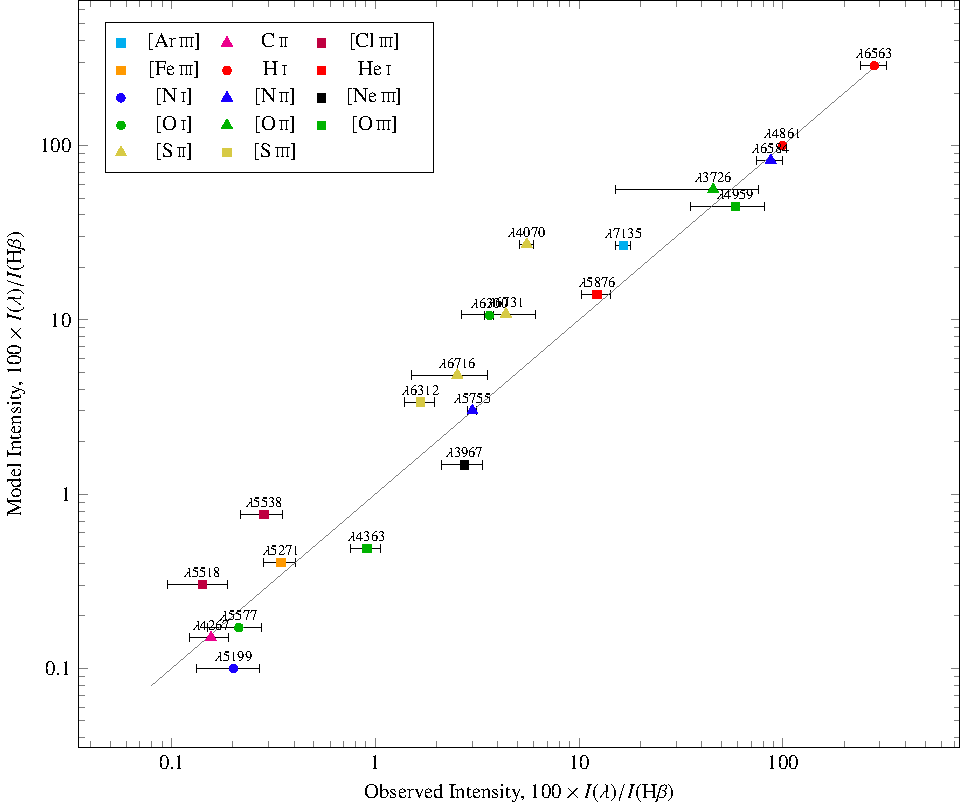
\includegraphics[]{ratios-figure-figure0.pdf}\\
    (b)\\
    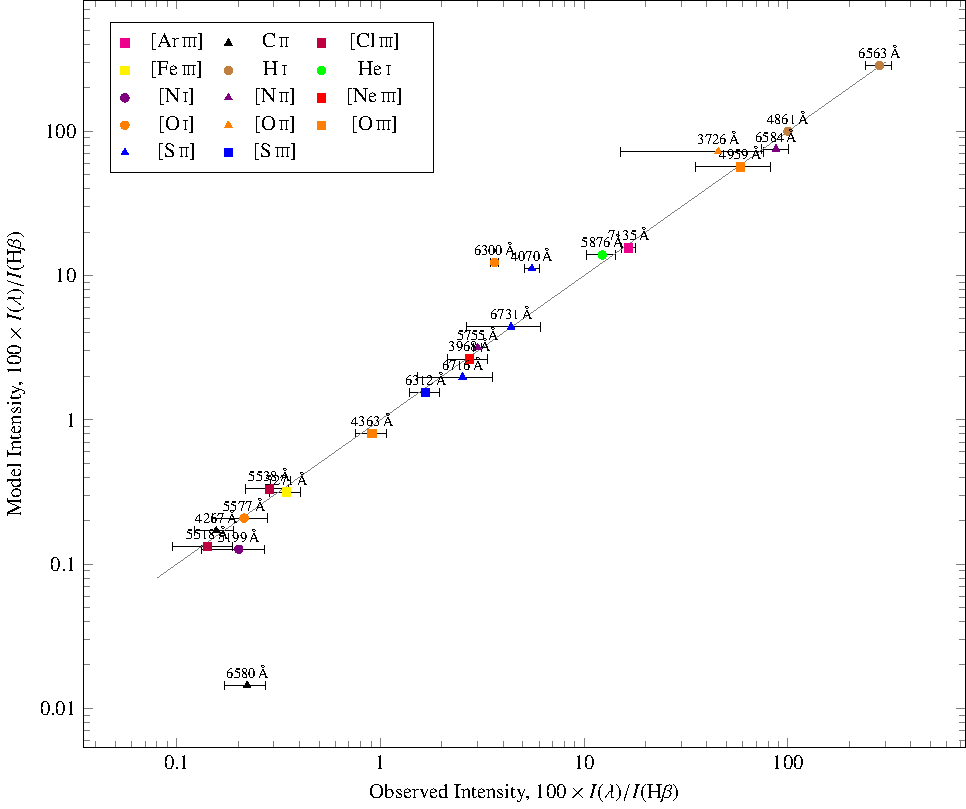
\includegraphics[]{ratios-figure-figure1.pdf}
  \end{tabular}
  \caption{Comparison between predicted and observed emission line fluxes 
    for photoevaporation models of HST~10 with 
    (a)~abundances as determined for the Orion Nebula by \protect\citet{2004MNRAS.355..229E},
    (b)~abundances determined for HST~10 in this paper.  
    The agreement in panel~(b) is much better, but there are still notable discrepancies.
  }
  \label{fig:models}
\end{figure*}


  \begin{figure*}
    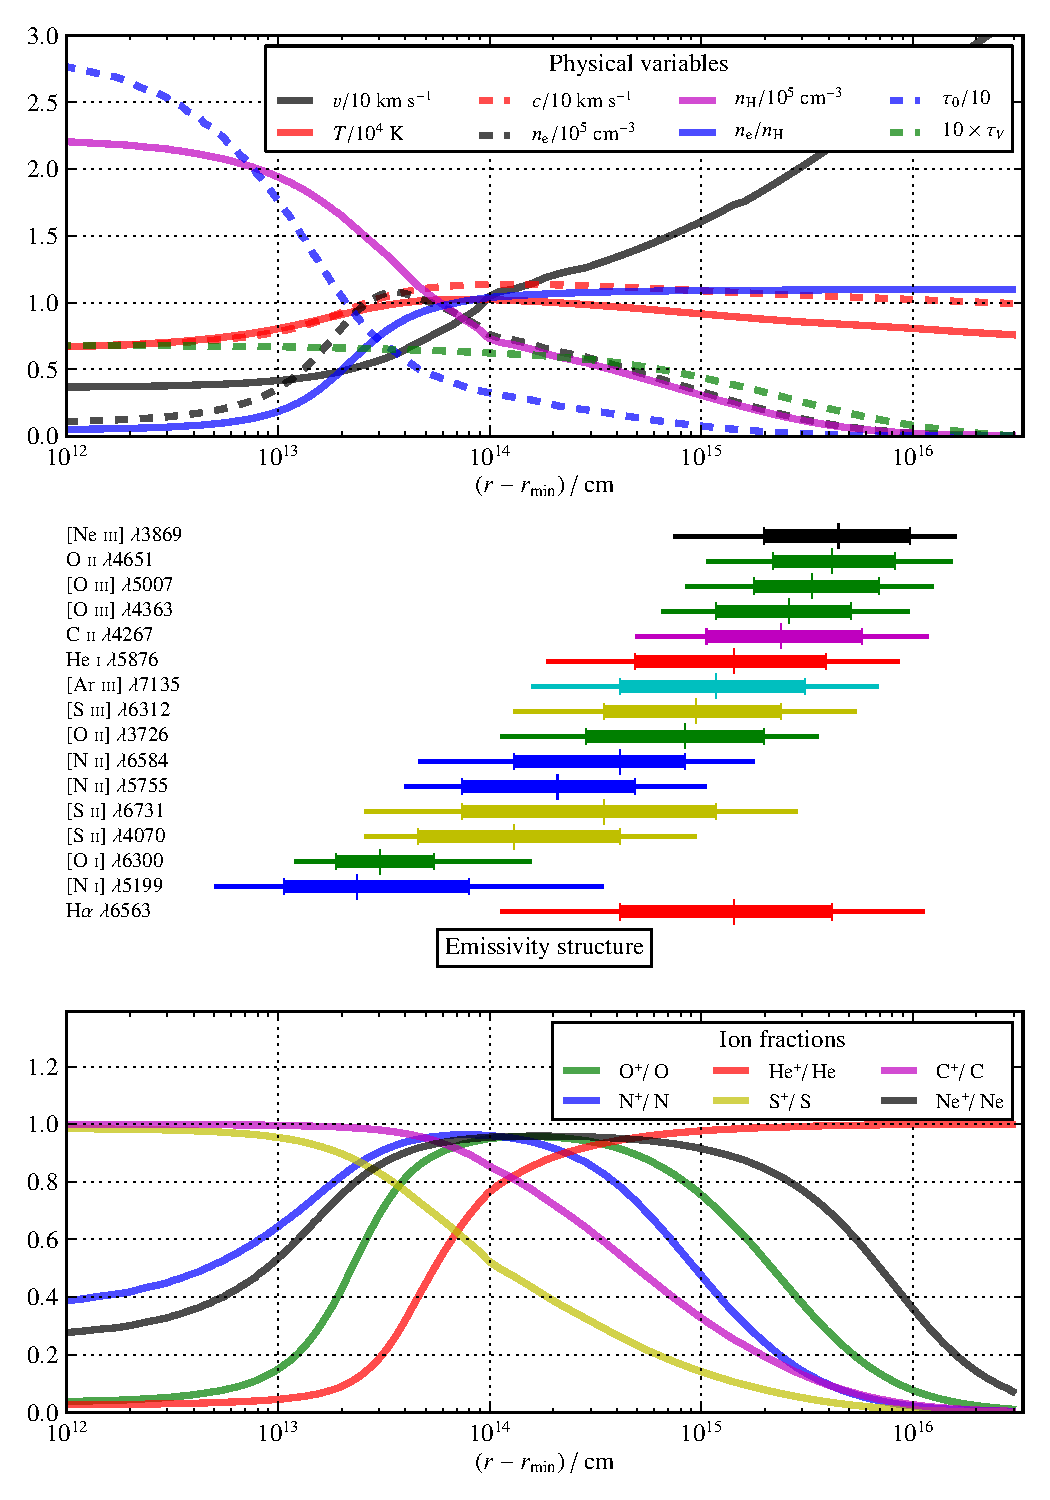
\includegraphics[width=0.75\linewidth]{model-structure-hst10-th30}
    \caption{Physical variables as a function of radius along a line at an angle of \(\theta = 30^{\circ}\) to the symmetry axis of our photoevaporation Model~B.    The radius \(r\) is measured from the center of curvature of the ionization front, shown on a logarithmic scale with respect to the deepest point in the model, \(r_{\mathrm{min}} = 3.5 \times 10^{15}\ \mathrm{cm}\).  (\textit{a}) Gas velocity in units of \(10\ \mathrm{km~s^{-1}}\) (solid black line).  Gas temperature, \(T\), in units of \(10^4\ \mathrm{K}\) (solid red line).  Isothermal sound speed, \(c\), in units of  \(10\ \mathrm{km~s^{-1}}\) (dashed red line).  Electron density, \(n_{\mathrm{e}}\), in units of \(7 \times 10^4\ \mathrm{cm^{-3}}\) (dashed black line).  Total hydrogen density, \(n_{\mathrm{H}}\), in units of  \(7 \times 10^4\ \mathrm{cm^{-3}}\) (solid purple line).  Electron fraction, \(n_{\mathrm{e}}/n_{\mathrm{H}}\) (solid blue line).  Lyman limit optical depth (divided by 10), measured from the ionizing source, which is located off the graph at \(r =  6.32 \times 10^{17}\ \mathrm{cm}\) (dashed blue line).  (\textit{b}) Fraction of singly ionized oxygen, \(\mathrm{O^{+}/O}\) (solid green line).  Fraction of singly ionized nitrogen, \(\mathrm{He^{+}/He}\) (solid yellow line).  Fraction of singly ionized sulfur, \(\mathrm{S^{+}/S}\) (dashed yellow line).  Fraction of singly ionized carbon, \(\mathrm{C^{+}/C}\) (solid purple line).  Results for other angles and abundance sets are similar, except with densities that scale roughly as \(\cos^{1/2}\theta\), and temperatures that tend to decrease slightly with \(\theta\) and with increased metal abundances.}
    \label{fig:model-structure}
  \end{figure*}


We have calculated dynamic photoevaporation models of HST~10, 
using the procedure outlined in \S~6 of \citet{Mesa-Delgado:2012}. 
The parameters for the models are shown in Table~\ref{tab:model:pars}. 
As compared with 177-341 (HST~1), which was modeled in \citet{Mesa-Delgado:2012},
HST~10 receives a roughly ten times smaller ionizing flux
and is roughly twice as large. 
Since \(F \propto n^2 r\) for recombination-dominated photoevaporation flows \citep{1990ApJ...354..529B, 2001RMxAC..10...57H},
this implies that the densities in HST~10 should be \(\simeq 5\) times smaller
and the ionization parameter \(\simeq 2\) times smaller than in HST~1. 

Two different abundance sets were used in the models.  
The first (Model~A) is the standard Orion gas phase abundance set, 
as determined by \cite{2004MNRAS.355..229E}.
The second (Model~B) is the set of abundances determined in this paper by empirical means, 
see Table~3. 
The resultant spectrum is shown in Figure~\ref{fig:models} for the two cases. 
It can be seen that the \citeauthor{2004MNRAS.355..229E} abundances 
produce very large discrepancies between the observed and predicted line fluxes 
(panel a). 
In particular, all Sulfur, Argon and Chlorine lines are too strong in the model 
by a factor of 3 to 10, 
whereas, \oiii{} 4363~\AA{} is too weak, indicating that the model temperature 
is too low in the highly ionized regions.
On the other hand, the \nii{} lines are well-reproduced y this model. 

The situation is much improved by using the Model~B abundances (panel b),
although serious discrepancies remain.  
The sulfur line fluxes are now in good agreement with the observations,
with the notable exception of the \sii{} 4070~\AA{} auroral line,
which is still 3 times too strong in the model. 
The \oi{} 6300~\AA{} shows a similar behaviour, being too strong by a factor of 4. 
These two lines, together with the \nii{} 5755~\AA{} auroral line, 
show the strongest contrast between the proplyd and the background nebula,
and hence are measured with a relatively small uncertainty,
making the disagreement highly significant. 
The \nii{} lines do not agree with Model~B so well as they do with Model~A, 
but the agreement is still fair given the uncertainties. 
The remaining disagreement is with the [\ion{N}{1}] 5199~\AA{} line,
but this is to be expected since the line arises through fluorescence in neutral gas
\citep{Ferland:2012},
whereas the model extends only to a hydrogen ionization fraction of 0.1 
and therefore misses part of the [\ion{N}{1}]-emitting zone.

It is not particularly surprising that the empirically determined abundances
do not reproduce the observed fluxes when used in our physical proplyd model. 
The same was seen in the case of HST~1,
where it was argued that the strong gradients in temperature and density,
both with and between ionization zones,
invalidated the empirical one-zone or two-zone approaches for analysing the spectrum.
However, in that case it was possible to find a different set of abundances for the model
that succeded in reproducing the observed spectrum to a high precision. 
Unfortunately, we have been unable to find such a satisfactory model for HST~10. 
Initial attempts to adjust the abundances have resulted in models that fit the observations 
\emph{worse} than Model~B does. 

The two most discrepant lines, \oi{}~6300~\AA{} and \sii{} 4070~\AA{} have 
a considerable overlap in their zones of emission.  
All the \oi{} emission, and roughly half of the \sii{} 4070~\AA{} arises 
from partially ionizes gas at the ionization front itself.
If the temperature of this gas is overestimated in the models, 
then the discrepancy could be explained. 
With the standard Orion dust properties that we are using in all the models
\citep{1991ApJ...374..580B},
photoelectric emission from dust grains provides up to 15\% of the heating
in this zone. 
Since there is some evidence that dust is depleted in the proplyd flows
\citep{2001ApJ...561..830G}, it may be feasible to reduce this heating,
which is an avenue that will be explored in future work. 


\bibliographystyle{mn2e}
\bibliography{BibdeskLibrary}


\end{document}
